\documentclass[12pt,a4paper]{article}
\usepackage[latin1]{inputenc}
\usepackage{float}
\usepackage{amsmath}
\usepackage{amsfonts}
\usepackage{amssymb}
\usepackage{graphicx}
\usepackage[hidelinks]{hyperref}
\usepackage{changepage}
\usepackage{subfig}
\usepackage{placeins}



\author{Davide Cocco - 944122\\
	Marco Gasperini - 944922}
\date{A.Y. 2019/2020 - Prof. Di Nitto Elisabetta}


\title{
	\textbf{\Huge{SafeStreets}} \\
	\large Design Document
}

\begin {document}

	\begin{figure}
		\centering
		
\includegraphics[width=1.0\linewidth]{Images/polimi.jpg}
	\end{figure}

	\maketitle
	\newpage
	\tableofcontents
	\newpage

\section{INTRODUCTION}
\subsection{Purpose}
This \texttt{Design Document (DD)} for the SafeStreets software will provide a functional description of the system by describing its architecture. 
It will eventually by used by the development team as a blueprint to guide the engineering of the application.
\subsection{Scope}
The main objective of the S2B will be assisting (thus not substituting) authorities and officers in handling traffic violations though a crowd-sourced platform in which civilians can participate. 
A mobile application will allow users, both civilians and officers, to report violations through the use of the camera and the GPS, sending the data to authorities who will process such reports. 
Law enforcement will be aided by a data mining system which will produce relevant data about the registered violations, and the S2B will be able to automatically compile a ticket and send it to
the municipality's VLA as soon as an officer personally convalidates a violation.
\subsection{Definitions, Acronyms, Abbreviations}
\subsubsection{Definitions}
\begin{itemize}
\item \texttt{Violation | Offence:} we will strictly refer to any kind of static traffic violation, especially parking violations. 
\item \texttt{Authority:} a law enforcement authority which is manages traffic violations, it could be the local police, the traffic wardens etc. We will refer with this term also to the personnel which operates the web application in the authorities' headquarters.
\item \texttt{User:} refers to the users of the mobile application, that is officers and civilians.
\end{itemize}
\subsubsection{Acronyms}
\begin{itemize}
\item \texttt{S2B:} software to be.
\item \texttt{HFVZ:} high violation frequency zone.
\item \texttt{GPS:} Global Positioning System.
\item \texttt{GDPR:} General Data Protection Regulation.
\item \texttt{DW:} data warehouse.
\item \texttt{VLA:} Vehicle Licensing Authority.
\item \texttt{RACS:} Reliable Array of Cloned Services.
\end{itemize}
\subsubsection{Abbreviations}
\begin{itemize}
	\item {[Gn]}: n-goal.
	\item {[Rn]}: n-requirment.
	\item {[Dn]}: n-domain assumption
	\item {App}: application.
\end{itemize}
\subsection{Revision History}
\subsection{Reference Documents}
\subsection{Document Structure}
\begin{itemize}
\item \textbf{Introduction}: includes the purpose and scope of the document along with some relevant definitions and acronyms used throughout the document.
\item \textbf{Architectural design}: this section is focused on the main components used for this system and the relationship between them, providing information about their
deployment and how they operate. it also focuses on the architectural styles and the design patterns adopted for designing the system.
\item \textbf{User interface design}: this section provides an overview on how the User Interface will look like, but it will be omitted due to the presence of this chapter in the RASD.
\item \textbf{Requirements traceability}: in this sections the requirements highlighted in the RASD document will be associated with the design elements explained in this document.
\item \textbf{Implementation, integration and test plan}: in this section we identify the order in which we plan to implement the subcomponents of the system and the order in which we plan to
integrate and test them.
\end{itemize}
\section{ARCHITECTURAL DESIGN}
\subsection{High level overview}
			\begin{figure}[H]
				\centering
					\begin{adjustwidth}{-25mm}{-25mm}
					        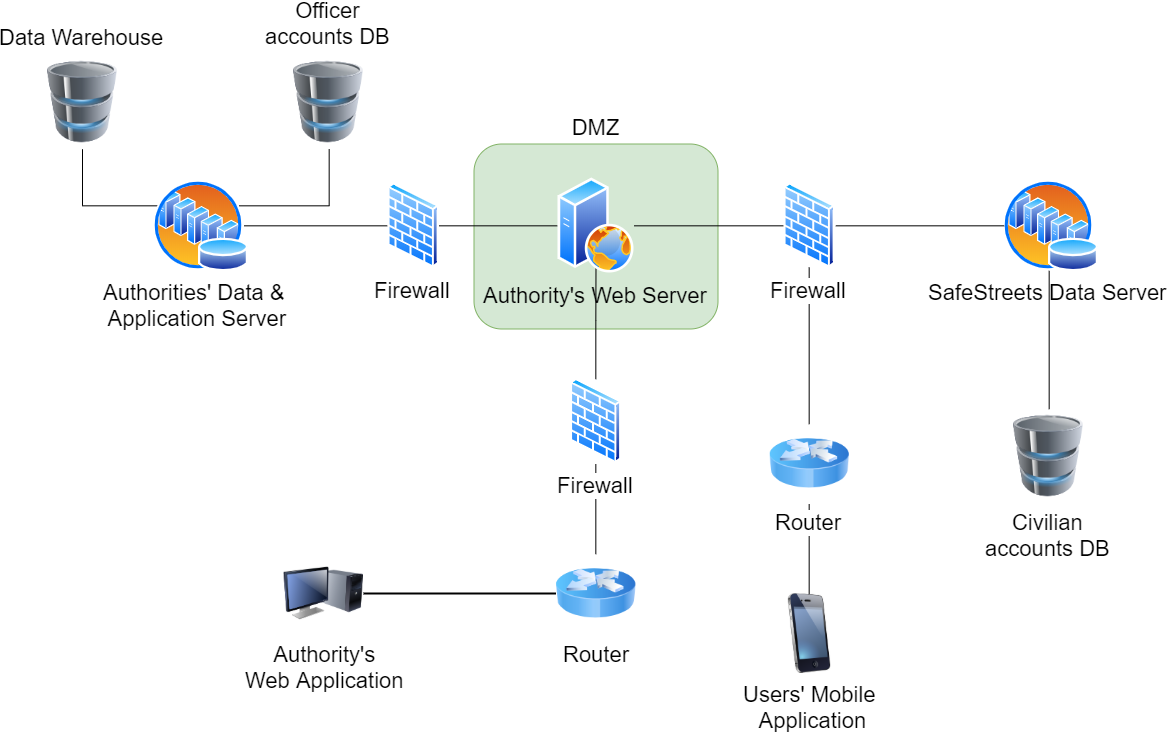
\includegraphics[width=.9\paperwidth,keepaspectratio]{Images/highlevel}
					\end{adjustwidth}
				\caption{Figure 1: High Level Structure}
			\end{figure}
The three logical layers of the S2B will be allocated this way:
\begin{itemize}
\item \textbf{Presentation layer:} the clients installed both at the authority's web application and at the users' mobile application. The mobile application sends its report to the authority's web server, which also manages receiving the processed data from the authorities' data server
and spreading it to the users and the authority's client. 
\item \textbf{Application layer:} each authority owns an application server in a DMZ, which hosts its logic that is customizable by an API to handle different jurisdictions' needs. 
\item \textbf{Data layer:} municipalities hold a data server which collects reports from all the authorities' data servers and distributes the processed data to be visualized on the clients. This data server also holds all the officers' data added by the authorities. 
Moreover, a RACS of data server at SafeStreets headquarters serves all registrations and logins from civilians, and also bans requested from the authorities to discourage wrong usages of the application.
\end{itemize}
\subsection{Component view}
The following diagrams illustrate the system components and the interfaces through which they interact to fullfil their functionalities. The diagram is focused on the application tier, so the remaining tiers (the presentation tier and the data tier) are shown as black-box.
First we have done a distinction between Client side and Server side:
\begin{itemize}
\item The Client side is composed by two components, \textit{Web Application} and \textit{Mobile Application}. The first is referred to the Authorities client, latter to the User client (Civilian and Officer).
\item The Server side is composed of three main components: \textit{Authorities Web Services} that manages, throught \textit{AuthoritiesWebServices} interface, on server side, the authorities client; the other two services are \textit{Civilian Mobile Services} and \textit{Officer Mobile Services} that manage throught two distinct interfaces the \textit{Mobile Application}.
\end{itemize}
\begin{figure}[H]
		\centering
			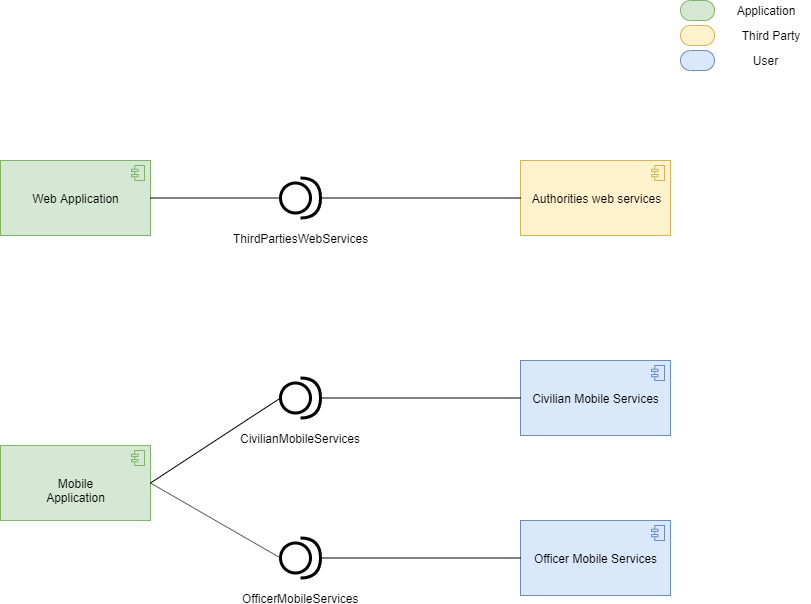
\includegraphics[width=1.0\linewidth]{Images/ComponentDiagram}
		\caption{Figure 2: Component diagram}
\end{figure}

\subsection{Deployment view}
\subsection{Runtime view: You can use sequence diagrams to describe the way components interact to accomplish specific tasks typically related to your use cases}
\subsection{Component interfaces}
\subsection{Selected architectural styles and patterns: Please explain which styles/patterns you used, why, and how}
\subsection{Other design decisions}
\section{USER INTERFACE DESIGN: Provide an overview on how the user interface(s) of your system will look like; if you have included this part in the RASD, you can simply refer to what you have already done, possibly, providing here some extensions if applicable.}
\section{REQUIREMENTS TRACEABILITY: Explain how the requirements you have defined in the RASD map to the design elements that you have defined in this document.}
\section{IMPLEMENTATION, INTEGRATION AND TEST PLAN: Identify here the order in which you plan to implement the subcomponents of your system and the order in which you plan to integrate such subcomponents and test the integration.}
\section{EFFORT SPENT}
\begin{itemize}
\item {Davide Cocco}
 \begin{center}
			\begin{tabular}{| c | l | c |}
				\hline
				\textbf{Day} & \textbf{Subject} & \textbf{Hours} \\ \hline
				Total & & 22.5 \\ \hline
			\end{tabular}
		\end{center}
\item {Marco Gasperini}
\begin{center}
			\begin{tabular}{| c | l | c |}
				\hline
				\textbf{Day} & \textbf{Subject} & \textbf{Hours} \\ \hline
				Total & & 19.5 \\ \hline
			\end{tabular}
\end{center}
\end{itemize}
\section{References}

\end {document}